% ||||||||||||||||||||||||||||||||||||||||
% |||||| 5.X Symmetron domain walls ||||||
% ||||||||||||||||||||||||||||||||||||||||

% -------------------------------------------------
% labels: \label{[type]:pertwalls:untitled1:[name]}
% -------------------------------------------------


%%%%%%%%%%%%%%%%%%%%%%%%%%%%%%%%%%%%%%%%%%%%%%%%%%%%%%%%%%%%%%%%%%%%%%%%%%%%%
% \newcommand{\eqregimenum}[1]{{\footnotesize{\textsf{\textbf{({#1})}}}}} 
\newcommand{\eqregimenum}[1]{{\tiny{\textsf{\textbf{(#1)}}}}}
%%%%%%%%%%%%%%%%%%%%%%%%%%%%%%%%%%%%%%%%%%%%%%%%%%%%%%%%%%%%%%%%%%%%%%%%%%%%%



We specify our example even further. The \nc{symmetron effective potential}[some sec.] is designed to provoke a phase transition at conformal time $\tau_\ast$, or scale factor $a_\ast$. Inserting this \nc{into Eq. XX}, we find that the surface tension of a thin symmetron domain wall is
\begin{equation}
    \sigma = \sigma_\infty \bclosed{1 -\pclosed{a_\ast/a}^3 }^{3/2},
\end{equation}
where $\sigma_\infty = 4\sqrt{2}/3\, \mu^3/\lambda$ is the asymptotic (``true'') surface energy density. 

From here it becomes advantagous to introduce some new, dimensionless variables (or dimensions). We will use $s\equiv \tau/\tau_\ast$ as our time variable, and $u=p\tau_\ast$ as the eigenvalue, when it comes to that. In a universe with $a = a_\ast s^\alpha$, the surface tension goes as $\sim {(1-s^{-3\alpha})}^{3/2}$, thus
\begin{equation}
    \frac{\sigma '}{\sigma} = \frac{1}{\sigma}\dv{\sigma}{s} = \dv{\ln{\sigma}}{s} = \frac{9\alpha}{2s\pclosed{s^{3\alpha} -1 }}
\end{equation}
Finally, the equation of motion for the wall normal coordinate is
\begin{equation}\label{eq:pertwalls:untitled1:eom_final}
    \epsilon'' + \left(  \frac{3\alpha}{s}  + 2 \gamma(s)\right)\epsilon' + u^2\epsilon = 0; \quad \gamma(s)\equiv \frac{9\alpha}{4 s \left( s^{3\alpha}-1 \right)}.
\end{equation}
From hereon, we express the function in terms of $s$ and $u$, i.e.~$\epsilon_u(s)$.



\subsection{Solution for $\alpha=2$}
    This project only truly experiments in a universe with, and only with, homogeneous matter distribution, i.e.~$\alpha=2$ and $\Omega\ped{m0}=1$. Generalisation of the following to other $\alpha$ should in principle be trivial, but at some point we require $\alpha\geq 1/3$, and so a different analysis would be required for smaller $\alpha$.

    So, restricting our discussion to $\alpha=2$, we continue with the planar domain wall placed parallel to the $xy$-plane, spontaneously formed at symmetry break, $s=1$. Assume an initial perturbation of amplitude $\epsilon_\ast$ was given to the wall, whose spatial part satisfies $(\partial_x^2 + \partial_y^2)\sppt(x,y)= -p^2 \sppt(x,y)$, giving the ``scale'' of the perturbation $p$. With initial conditions $\epsilon_u(s=1)=\epsilon_\ast$ and $\epsilon_u'(s=1)=0$, we shall solve
    \begin{equation}\label[eq]{eq:pertwalls:untitled1:eom_eps_s_MD}
        \epsilon'' + \left( \frac{6}{s}  +\frac{9}{2s\left(s^6-1\right)} \right) \epsilon' + u^2 \epsilon = 0
    \end{equation}
    analytically in two regimes, and sow these solutions together in the region where they overlap. For notational ease, we write $\epsilon_u(s) = \epsilon_\ast e(s)$.
    

    \paragraph{Shortly after symmetry breaking.} %
    We begin by solving the equation of motion for $s\sim 1$. As our equation has a singularity at $s=1$, the natural way to go is through a Laurent expansion around this point of the damping term in~\cref{eq:pertwalls:untitled1:eom_eps_s_MD}. We find 
    \begin{equation}
        \frac{6}{s}  +\frac{9}{s\left(s^6-1\right)} = \frac{3}{2} (s-1) + \frac{3}{4} + \frac{29}{8}(s-1)- \frac{93}{16} {(s-1)}^2 + \BigO{{(s-1)}^3}.
    \end{equation}
    Now $e(s)$ is also subject to an expansion around $s=1$;
    \begin{equation}
        e(s) = \bclosed{ 1 + c_1 (s-1) + c_2 {(s-1)}^2 + c_3 {(s-1)}^3 + \dots }.
    \end{equation}
    % We immediately see that the initial condition 
    When put together, we get a polynomial in $(s-1)$ on the left-hand side of~\cref{eq:pertwalls:untitled1:eom_eps_s_MD}, for which all coefficients must vanish. %Solving the system of equations gives $c_1 = 0$, $c_2 =-q^2/5$ and $c_3 = q^2/35$. Thus,
    We solve the system of equations for $\cclosed{c_1,c_2, c_3} $ and find 
    \begin{equation}\label[eq]{eq:pertwalls:untitled1:eps_s_I_MD}
        e^{\text{\eqregimenum{I}}}(s) = \bclosed{ 1 - \frac{u^2}{5} {(s-1)}^2 + \frac{u^2}{35} {(s-1)}^3 } + \BigO{\pclosed{s-1}^4}.
    \end{equation}



    \paragraph{Adiabatic evolution.} %
    The damping term $2\gamma(s)= 9/(2s(s^6-1))$ initially changes extremely rapidly from very large values, before it becomes very small compared to $3a'/a=6/s$. We expect the solution to quickly approach that of~\cref{eq:pertwalls:untitled1:eom_eps_s_MD_simple} as $s\gg 1$. 
    % For $s\gg 1$, the damping term $\gamma(s) = 9/(2 s(s^6-1))$ in the eom for $\epsilon$ becomes subdominant \comment{check plag. Julian}, and asymptotically the solution is $s^{-2}\cclosed{c \sphBessel[2](qs) + d \sphNeumann[2](qs)  }$. 
    Said damping term is not completely negligible, however, as it causes a \emph{damping envelope} that is considered much like in the case of a damped harmonic oscillator, writing
    \begin{equation}\label[eq]{eq:pertwalls:untitled1:eps_s_II_MD_w}
        e^{\text{\eqregimenum{II}}}(s) \simeq   w(s) \cdot \exp{ - \integ{t}[][s] \gamma(t) }.%; \quad w(s) = \frac{c\sphBessel[2](qs) + d \sphNeumann[2](qs)}{s^2}.
    \end{equation}
    Employing this ansatz in the eom gives
    \begin{equation}
        w'' + \frac{6}{s} w' + \pclosed{q^2 - \theta(s) }w = 0; \quad \theta(s) = \gamma'(s) + \gamma^2(s) + \frac{6}{s}\gamma (s),
    \end{equation}
    whose solution is $w(s) \simeq s^{-5/2}\Sylindrical[-5/2](us)$ %
    % \begin{equation}\label{eq:pertwalls:untitled1:w_of_s_undet}
    %     w(s) \simeq s^{-5/2}\Sylindrical[-5/2](us)  \simeq s^{-5/2} \cclosed{ A \Bessel[-5/2](us) + B \Neumann[-5/2](us) }
    % \end{equation}
    when the phase shift introduced by $\theta(s)$ is negligible. % and $A$ and $B$ are constants.%
    {\footnote{In fact, it is possible to show that $\lim_{u\to \infty}{\bclosed{\sqrt{u^2-\theta(1+u^{-1})}-u} /u }= \sqrt{19}/4 -1 \approx 0.09$.}} %
    Now, we find that $\exp{-\integ{t}[][s] \gamma(t)} =s^{9/2} (s^6-1)^{-3/4}  \cdot \text{constant}$. Thus
    \begin{equation}
        e^{\text{\eqregimenum{II}}}(s) \simeq \frac{ A \Bessel[-5/2](us) + B \Neumann[-5/2](us) }{s^{5/2}} \frac{s^{9/2}}{{(s^6-1)}^{3/4}},
    \end{equation}
    where $A$ and $B$ are constants to be determined.

    \paragraph{Complete evolution.} %
    %We have obtained solutions for $\epsilon(s)$ in two regimes. We say that $\epsilon(s)$ obeys~\cref{eq:pertwalls:untitled1:eps_of_s_first} for $s \in [1, s\ped{sow}]$ and~\cref{eq:pertwalls:untitled1:eps_of_s_second_general} for $s\in [s\ped{sow}, \infty)$, where $s\ped{sow}$ is close to, but strictly larger than 1. We choose $s\ped{sow}=1+q^{-1}$ since only \cringe{causally conntected modes}, for which $q\gg 1$, are of interest to us. 
    We use a computer algebra system, namely \textit{SageMath}~\citep{sagemath}, to determine $A$ and $B$ from the system of equations
    \begin{equation}
        \begin{split}
            e^{\text{\eqregimenum{I}}}(s=s\ped{sow}) &= e^{\text{\eqregimenum{II}}}(s=s\ped{sow}) \\
            % \dv{e^{\text{\eqregimenum{I}}}}{s} \bigg|_{s=s\ped{sow}}&= \dv{e^{\text{\eqregimenum{II}}}}{s} \bigg|_{s=s\ped{sow}}
            {e^{\text{\eqregimenum{I}}}}'(s=s\ped{sow}) &= {e^{\text{\eqregimenum{II}}}}'(s=s\ped{sow})
        \end{split}
    \end{equation}
    \comment{maybe put expressions in appendix?}
    where we choose $s\ped{sow}=1+u^{-1}$, since only subhorizon modes, $u\gg 1$, are of interest. Now,
    \begin{equation}\label{eq:pertwalls:untitled1:eps_s_complete_MD}
        \epsilon_u(s) =  \epsilon_\ast \cdot \begin{cases}
            e^{\text{\eqregimenum{I}}} (s),  & s \leq s\ped{sow}, \\
            e^{\text{\eqregimenum{II}}}(s),  & s \geq s\ped{sow}.
        \end{cases}
    \end{equation}
    In~\cref{fig:pertwalls:untitled1:demo001} we demonstrate how this solution looks like for arbitrary $u$, in the different steps described above. \comment{Should include solution in the case where surface tension is constant.}
    %%%%%%%%%%%%%%%%%%%%%%%%%%%%%%%%%%%%%%%%%%%%%%%%%%%%%%%%%%%%%%%%%%%%%%%%%%%%
    %%%%%%%%%%%%%%%%%%%%%%%            FIGURE            %%%%%%%%%%%%%%%%%%%%%%%
    %%%%%%%%%%%%%%%%%%%%%%%%%%%%%%%%%%%%%%%%%%%%%%%%%%%%%%%%%%%%%%%%%%%%%%%%%%%%
    \begin{figure}
        \centering
        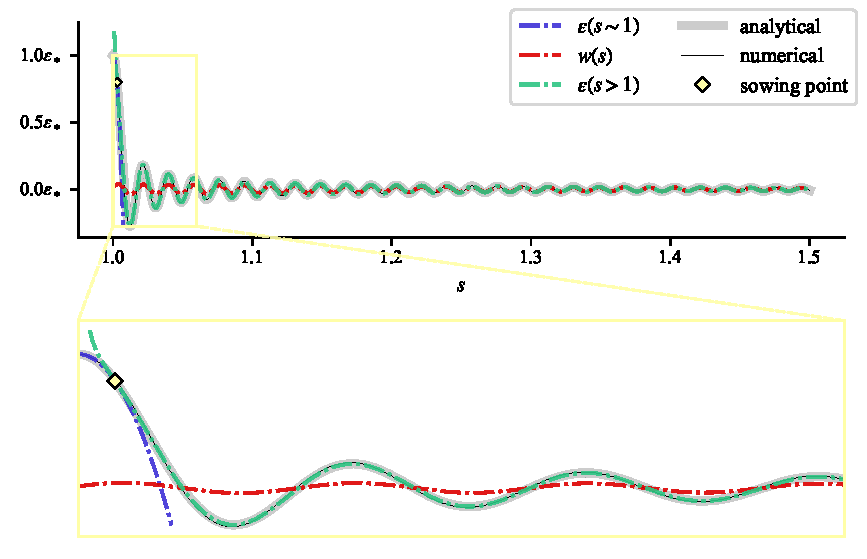
\includegraphics[width=\linewidth]{demo001.pdf}
        %%%%%%%%%%
        \caption{Schematic demonstrating how the analytical solution to the eom for $\epsilon_u(s)$.}  
        \label[fig]{fig:pertwalls:untitled1:demo001}
    \end{figure}
    %%%%%%%%%%%%%%%%%%%%%%%%%%%%%%%%%%%%%%%%%%%%%%%%%%%%%%%%%%%%%%%%%%%%%%%%%%%%

    
    

    

\subsection{\tmptitle{Review}}
    %%%%%%%%%%%%%%%%%%%%%%%%%%%%%%%%%%%%%%%%%%%%%%%%%%%%%%%%%%%%%%%%%%%%%%%%%%%%
    %%%%%%%%%%%%%%%%%%%%%%%            FIGURE            %%%%%%%%%%%%%%%%%%%%%%%
    %%%%%%%%%%%%%%%%%%%%%%%%%%%%%%%%%%%%%%%%%%%%%%%%%%%%%%%%%%%%%%%%%%%%%%%%%%%%
    \begin{figure}
        \centering
        \includegraphics[width=\linewidth]{dummy_normal.png}
        %%%%%%%%%%
        \caption{Demonstration of the effect of changing scale parameter $u=p\tau_\ast$.}  
        %\label[fig]{fig:pertwalls:untitled1:932434t}
    \end{figure}
    %%%%%%%%%%%%%%%%%%%%%%%%%%%%%%%%%%%%%%%%%%%%%%%%%%%%%%%%%%%%%%%%%%%%%%%%%%%%
    For the time being, let us assume~\cref{eq:pertwalls:untitled1:eps_s_complete_MD} is a good description of the perturbed symmetron wall. We immidiately see that the initial amplitude $\epsilon_\ast$ can be factored out and does not affect the evolution. We keep in mind that this parameter is still important for the validity of the eom that requires $\epsilon_\ast \ll \tau_\ast$. 
    The scale parameter $u=p\tau_\ast$ determines the frequency of oscillations. We observe that this result \checkthis{is completely independent of $\tau_\ast$.}
    
    \paragraph{Scaling.} %
    It turns out that if plotted over the time variable $t\equiv u(s-1)=p(\tau-\tau_\ast)$, the solution in~\cref{eq:pertwalls:untitled1:eps_s_complete_MD} is \checkthis{equal up to normalisation in $\epsilon_\ast$}

    \subsubsection{Spatial part}
        We need to adress the until now neglected function $\mathscr{E}(x,y)$. It is a solution to
        \begin{equation}
            \pdv[2]{\mathscr{E}}{x} + \pdv[2]{\mathscr{E}}{y} = -p^2 \mathscr{E},
        \end{equation}
        and it is natural to demand $\max{\abs{\mathscr{E}}} = 1$ and $\mathscr{E}\in\Real$. \checkthis{The general solution to this equation is $\eu[\im (p_x x + p_y y)]$}





\subsection{Asymmetron domain walls}
    Let us have a quick peek at what would happen if introducing asymmetry in the potential. We consider a constant surface tension and vacuum energy densities. In the thin-wall limit, we should be able to use 

%%%%%%%%%%%%%%%%%%%%%%%%%%%%%%%%%%%%%%%%%%%%%%%%%%%%%%%%%%%%%%%%%%%%%%%%%%%%
%%%%%%%%%%%%%%%%%%%%%%%%%%%%%%%%%%%%%%%%%%%%%%%%%%%%%%%%%%%%%%%%%%%%%%%%%%%%







% \comment{We find that $\lim_{q\to \infty}{\bclosed{q\ped{mod}(s\ped{sow})-q} /q }= \sqrt{19}/4 -1 \approx 0.09$ for $s\ped{sow}=1+q^{-1}$ and $q\ped{mod}(s) = \sqrt{q^2 -\theta(s)  }$.}





% For $s\gg 1$, the term $\gamma(s) = 9/(2 s(s^6-1))$ in the eom for $\epsilon$ is of order $\BigO{s^{-7} }$, and thus negligible. Completely ignoring this term gives a differential equation with the general solution $s^{-\tau} \cdot \cclosed{d_{1} \Bessel[\tau](qs) + d_{2} \Neumann[\tau](qs)  }$ where $\tau=(1-3\alpha)/2=-5/2$.
% \begin{equation}
%     \epsilon(s) = 
% \end{equation}









%%%%%%%%%%%%%%%%%%%%%%%%%%%%%%%%%%%%%%%%%%%%%%%%%%%%%%%%%%%%%%%%%%%%%%%%%%%%
%%%%%%%%%%%%%%%%%%%%%%%%%%%%%%%%%%%%%%%%%%%%%%%%%%%%%%%%%%%%%%%%%%%%%%%%%%%%
% \begin{draft}

% \paragraph{Not constant surface tension.} %
% We now let the surface tension of the domain wall be dependent of time. The variation of the action becomes slightly different, and the resulting equation of motion
% \begin{equation}
%     \ddot{\epsilon} + \pclosed{ 3\frac{\dot{a}}{a} + \frac{\dot{\sigma}}{\sigma} } \dot{\epsilon} + k^2 \epsilon = 0.
% \end{equation}
% A simple way to obtain this equation is to substitute $a\to \sigma^{1/3}a$ in the equations above.

% We assume an ideal situation in which SSB occurs at some conformal time $\eta_\ast$ in a universe where $a= a_\ast (\eta/\eta_\ast)^\alpha$. It is useful to introduce a dimensionsless time variable $s\equiv\eta/\eta_\ast$, s.s.~$a=a_\ast s^\alpha$, as well as a parameter $q\equiv k\eta_\ast$. The surface tension of a domain wall is computed from the Symmetron effective potential
% \begin{equation}
%     V\ped{eff} (\phi) = \frac{\lambda}{4} \phi^4 + \frac{\mu^2}{2} \left( \frac{\rho\ped{m}}{\mu^2 M^2} - 1\right) \phi^2 + V_0.
% \end{equation}
% We define the matter density at SSB to be $\rho\ped{m}|_{\eta=\eta_\ast}= \mu^2 M^2$. Since $\rho\ped{m}\propto a^{-3(1+w\ped{m})} = a^{-3}$, we get
% \begin{equation}
%     \rho\ped{m} = \mu^2 M^2 \left(a_\ast/a \right)^3 = \mu^2 M^2 \left(\eta_\ast/\eta \right)^{3\alpha} = \mu^2 M^2 s^{-3\alpha}.
% \end{equation}
% % \begin{align}
% %     \frac{\rho_s}{\rho_{s0}} &= \left(\frac{a}{a_0}\right)^{-3(1+w_s)}
% % \end{align}
% \blahblah The surface tension becomes
% \begin{equation}
%     \sigma = \sigma_0 \left(1 - s^{-3\alpha}\right)^{3/2}.
% \end{equation}
% Finally, the equation of motion for the wall normal coordinate $\epsilon n\^\mu$ is
% \begin{equation}\label{eq:pertwalls:untitled1:eom_final}
%     \epsilon'' + \left(  \frac{3\alpha}{s}  + 2 \gamma(s)\right)\epsilon' + q^2\epsilon = 0; \quad \gamma(s)= \frac{9\alpha}{4 s \left( s^{3\alpha}-1 \right)}.
% \end{equation}



% We assume the wall to be thin, and so the surface tension is given by

% \subsection{Solving the equation of motion in a matter dominated universe}
% We restrict our discussion to $\alpha=2$. The generalisation to $\alpha \geq 1/3$ is trivial \comment{in appendix, maybe?}. We shall solve~\cref{eq:pertwalls:untitled1:eom_final} in two regimes of $s$ and sow these solutions together. In the following, we neglect the spatial part of $\epsilon$, that which is subject to \comment{explain this}

% $\epsilon(\eta, x, y) =$

% % The field $\epsilon = \epsilon_q(s, x, y)$ 

% Consider a planar domain wall formed during SSB at spacetime position $X\^\mu= (\eta_\ast, x, y, z_0)$.
% Assume that such a formation induces a perturbation to the wall that moves the wall normal coordinate from $z_0$ to $z_0 + \epsilon_\ast$. This gives the initial condition $\epsilon(1)=\epsilon_\ast$ to the equation of motion for $\epsilon(s)$ with $\alpha=2$, namely
% \begin{equation}\label{eq:pertwalls:untitled1:eom_MD}
%     \epsilon'' + \left( \frac{6}{s}  +\frac{9}{s\left(s^6-1\right)} \right) \epsilon' + q^2 \epsilon = 0.
% \end{equation}
% The dimensionless variables are restricted $s\geq 1$ and $q\gg 1$ to ensure that SSB has happened and \rephrase{that the scale of the perturbation is subhorizon.}

% \paragraph{Shortly after symmetry breaking.} %
% We begin by solving the equation of motion for $s\sim 1$. As our equation has a singularity at $s=1$, the natural way to go is through a Laurent expansion around this point of the damping term in~\cref{eq:pertwalls:untitled1:eom_MD}. We find 
% \begin{equation}
%     \frac{6}{s}  +\frac{9}{s\left(s^6-1\right)} = \frac{3}{2} (s-1) + \frac{3}{4} + \frac{29}{8}(s-1)- \frac{93}{16} {(s-1)}^2 + \BigO{{(s-1)}^3}.
% \end{equation}
% Now $\epsilon(s)$ is also subject to an expansion around $s=1$;
% \begin{equation}
%     \epsilon(s) = \epsilon_\ast \cdot \bclosed{ 1 + c_1 (s-1) + c_2 {(s-1)}^2 + c_3 {(s-1)}^3 + \dots }.
% \end{equation}
% % We immediately see that the initial condition 
% When put together, we get a polynomial in $s-1$ on the left-hand side of~\cref{eq:pertwalls:untitled1:eom_MD}, for which all coefficients must vanish. %Solving the system of equations gives $c_1 = 0$, $c_2 =-q^2/5$ and $c_3 = q^2/35$. Thus,
% We solve the system of equations for $\cclosed{c_1,c_2, c_3} $ and find 
% \begin{equation}\label{eq:pertwalls:untitled1:eps_of_s_first}
%     \epsilon(s) = \epsilon_\ast \cdot \bclosed{ 1 - \frac{q^2}{5} {(s-1)}^2 + \frac{q^2}{35} {(s-1)}^3 } + \BigO{\pclosed{s-1}^4}, \quad s \gtrsim 1
% \end{equation}


% \paragraph{Later times.} %
% For $s\gg 1$, the damping term $\gamma(s) = 9/(2 s(s^6-1))$ in the eom for $\epsilon$ becomes subdominant \comment{check plag. Julian}, and asymptotically the solution is $s^{-2}\cclosed{c \sphBessel[2](qs) + d \sphNeumann[2](qs)  }$. Said damping term is not completely negligible, however, as it causes a \emph{damping envelope} that is considered much like in the case of a damped harmonic oscillator, writing
% \begin{equation}\label{eq:pertwalls:untitled1:eps_of_s_second_general}
%     \epsilon(s) \simeq \epsilon_\ast \cdot  w(s) \cdot \exp{ - \integ{t}[][s] \gamma(t) }.%; \quad w(s) = \frac{c\sphBessel[2](qs) + d \sphNeumann[2](qs)}{s^2}.
% \end{equation}
% Employing this ansatz in the eom gives
% \begin{equation}
%     w'' + \frac{6}{s} w' + \pclosed{q^2 - \theta(s) }w = 0; \quad \theta(s) = \gamma'(s) + \gamma^2(s) + \frac{6}{s}\gamma (s)
% \end{equation}
% whose solution is 
% \begin{equation}\label{eq:pertwalls:untitled1:w_of_s_undet}
%     w(s) \simeq s^{-5/2} \cclosed{ A \Bessel[-5/2](qs) + B \Neumann[-5/2](qs) }
% \end{equation}
% when the phase shift introduced by $\theta(s)$ is negligible and $A$ and $B$ are constants.%
% {\footnote{In fact, it is possible to show that $\lim_{q\to \infty}{\bclosed{\sqrt{q^2-\theta(1+q^{-1})}-q} /q }= \sqrt{19}/4 -1 \approx 0.09$.}} %
% Now, we find that $\exp{-\integ{t}[][s] \gamma(t)} =s^{9/2} (s^6-1)^{-3/4}  \cdot \text{const.}$, so in redefining the constants $A$ and $B$, we have
% \begin{equation}
%     \epsilon(s) \simeq \epsilon_\ast  \cdot \frac{ A \Bessel[-5/2](qs) + B \Neumann[-5/2](qs) }{s^{5/2}} \frac{s^{9/2}}{{(s^6-1)}^{3/4}}, \quad s \geq s\ped{sow}
% \end{equation}



% \paragraph{Putting it together.} %
% We have obtained solutions for $\epsilon(s)$ in two regimes. We say that $\epsilon(s)$ obeys~\cref{eq:pertwalls:untitled1:eps_of_s_first} for $s \in [1, s\ped{sow}]$ and~\cref{eq:pertwalls:untitled1:eps_of_s_second_general} for $s\in [s\ped{sow}, \infty)$, where $s\ped{sow}$ is close to, but strictly larger than 1. We choose $s\ped{sow}=1+q^{-1}$ since only \cringe{causally conntected modes}, for which $q\gg 1$, are of interest to us. We use a computer algebra system, namely \textit{SageMath}~\citep{sagemath}, to determine $A$ and $B$ in~\cref{eq:pertwalls:untitled1:w_of_s_undet} from the system of equations that comes from equating the right-hand sides of~\cref{eq:pertwalls:untitled1:eps_of_s_first} and~\cref{eq:pertwalls:untitled1:eps_of_s_second_general} with $s=s\ped{sow}$. 



% \begin{figure}[h]\label{fig:test}
%     \import{figs/}{demo001.tex}
% \end{figure}

% \begin{bullets}
%     \item We assume given values of $\epsilon_\ast$ and $q$
%     \item $A$ and $B$ are constants dep. on choice of $s\ped{sow}$ (and $q$)
%     \item Find a place to show the expressions for $A$ and $B$, maybe an attachment or appendix
%     \item Two free parameters: As we can see, changing the amplitude $\epsilon_\ast$ does not change the motion, but varying the wavenumber $q$ does
% \end{bullets}


% \begin{equation}
%     \epsilon_q(s, x, y) = \epsilon_\ast \cdot \begin{cases}
%         1(\dots) & 1 \leq s \leq s\ped{sow} \\
%         2 (\dots)  &s\ped{sow} \leq s < \infty \quad \mathcal{H}
%     \end{cases}
% \end{equation}


% \end{draft}
%%%%%%%%%%%%%%%%%%%%%%%%%%%%%%%%%%%%%%%%%%%%%%%%%%%%%%%%%%%%%%%%%%%%%%%%%%%%
%%%%%%%%%%%%%%%%%%%%%%%%%%%%%%%%%%%%%%%%%%%%%%%%%%%%%%%%%%%%%%%%%%%%%%%%%%%%







% \comment{We find that $\lim_{q\to \infty}{\bclosed{q\ped{mod}(s\ped{sow})-q} /q }= \sqrt{19}/4 -1 \approx 0.09$ for $s\ped{sow}=1+q^{-1}$ and $q\ped{mod}(s) = \sqrt{q^2 -\theta(s)  }$.}





% For $s\gg 1$, the term $\gamma(s) = 9/(2 s(s^6-1))$ in the eom for $\epsilon$ is of order $\BigO{s^{-7} }$, and thus negligible. Completely ignoring this term gives a differential equation with the general solution $s^{-\tau} \cdot \cclosed{d_{1} \Bessel[\tau](qs) + d_{2} \Neumann[\tau](qs)  }$ where $\tau=(1-3\alpha)/2=-5/2$.
% \begin{equation}
%     \epsilon(s) = 
% \end{equation}



